\section{Структура}
Структура входных данных(файла журнала) разнородна. Это может быть как стэк
вызовов функции языка javascript(несколько строк). Так и ошибки, вызова
функций языка perl. Так и отладочные сообщения о входящем запросе неправильного
формата. Все эти сообщения имеют принципиально разный формат, к тому же
некоторые имеют мета-информацию(временная отметка, важность и т.д.),
другие --- нет.

За счёт этого, даже сообщения об одной и той же ошибке могут совпадать
неполностью(различные временные отметки) или практически полностью несовпадать
--- информация об ошибке и длинный путь до файла.

Поэтому на первом этапе необходимо унифицировать сообщения об ошибках за счёт
замены мета-информации и дополнительных сведений на строковые константы:

\begin{example}[Замена мета-информации и доп. сведений]
UUID вида ACE088EB-ECA6-4348-905A-041EF10DBD53 можно заменить на строковую
константу вида UUID\_SUBSTITUTE.
\end{example}

\begin{example}[Замена мета-информации и доп. сведений]
ip-адрес вида 10.205.10.74 можно заменить на строковую
константу вида IP\_ADDRESS\_SUBSTITUTE.
\end{example}

После этого данные станет проще анализировать с помощью алгоритмов,
так как одинаковые ошибки будут совпадать, независимо от времени появления или
идентификатора запроса.

Для поиска и замены удобно использовать регулярные выражения, например:
\begin{center}
  \begin{itemize}
    \item
      \begin{verbatim}
        '(\d{16}-[-\w]*\b)', 'REQUEST_ID_SUBSTITUTE'
      \end{verbatim}
    \item
      \begin{verbatim}
        '([0-9A-F]){8}-[0-9A-F]{4}-[0-9A-F]{4}-
        [0-9A-F]{4}-[0-9A-F]{12}', 'UUID_SUBSTITUTE'
      \end{verbatim}
    \item
      \begin{verbatim}
        '\b(\d{1,3}\.){3}\d{1,3}\b', 'IP_ADDRESS_SUBSTITUTE'
      \end{verbatim}

    \item
      \begin{verbatim}
        '\w{3} \w{3} \d{1,2} \d{1,2}:\d{1,2}:
        \d{1,2} \d{4}', 'TIMESTAMP_SUBSTITUTE'
      \end{verbatim}
    \item
      \begin{verbatim}
        'line \d+', 'LINE_SUBSTITUTE'
      \end{verbatim}
  \end{itemize}
\end{center}

Такого рода пары(регулярное выражение, строковая константа) удобно хранить и
использовать. Регулярные выражения --- гибкий инструмент, поддерживаемый
практически всеми современными языками программирования.

Сами сообщения об ошибках можно представить в виде регулярных выражений.
Но зачем тогда делать первый этап преобразования входных данных? Теоретически
можно описать сообщение об ошибке регулярным выражением, но на практике
это регулярное выражение будет достаточно сложным и нечитаемым, поэтому
подготовка начальных данных сильно упрощает регулярные выражения, используемые
для выделения ошибки. Например следующий многострочный шаблон было бы
воспринимать человеку ещё сложнее, если бы, вместо строковых констант были бы
регулярные выражения:

\begin{center}
  \begin{verbatim}
"""JavaScript\.\ TypeError\:\ Object\
\#\<t\>\ has\ no\ method\ \'Ukraine\'
\ \ \ \ at\ Object\.blocks\.b\-counters\
_\_gemius\ \(web3\_exp\/pages\-desktop\/
search\/\_search\.all\.priv\.js\:POSITION\_SUBSTITUTE\)
\ \ \ \ at\ Object\.\[object\ Function\]\
.Object\.toString\.call\.e\.\(anonymous\ function\)\
\[as\ b\-counters\_\_gemius\]\ \(web3\_exp\/pages\
-desktop\/search\/\_search\.all\.priv\.js\:POSITION\_SUBSTITUTE\)
\ \ \ \ at\ Object\.blocks\.b\-counters\.blocks\.b\-cntrs\
\(web3\_exp\/pages\-desktop\/search\/\_search\.all\
.priv\.js\:POSITION\_SUBSTITUTE\)
\ \ \ \ at\ Object\.\[object\ Function\]\.Object\
.toString\.call\.e\.\(anonymous\ function\)\
\[as\ b\-counters\]\ \(web3\_exp\/pages\-desktop\/
search\/\_search\.all\.priv\.js\:POSITION\_SUBSTITUTE\)
\ \ \ \ at\ Object\.\[object\ Function\]\.Object\.toString\.
call\.e\.\(anonymous\ function\)\ \[as\ b\-page\]\
\(web3\_exp\/pages\-desktop\/search\/\_search\.all\
.priv\.js\:POSITION\_SUBSTITUTE\)\ at\
\/db\/BASE\/upper\-SHARD\_SUBSTITUTE\/arkanavt\/report\
/lib\/YxWeb\/Util\/Template\/JS\.pm\ LINE\_SUBSTITUTE\.\
\(Object\.blocks\.b\-page\ \(web3\_exp\/pages\-desktop\/search\/
\_search\.all\.priv\.js\:POSITION\_SUBSTITUTE\)\)\n\Z""",
  \end{verbatim}
\end{center}

Также использование дополнительных регулярных выражений в шаблонах, приводит
к падению производительности, увеличивает вероятность ошибки при подсчёте
статистики и усложняет автоматическое выделение новых шаблонов.

Для подсчёта статистики используется достаточно простая структура --- пара
(шаблон, количество совпадений). Это один из ключевых моментов, позволяющих
легко масштабировать приложение, реализующее алгоритм,
с помощью модели MapReduce.

\section{Архитектура}

Для реализации поставленных на этапе анализа требований задачи были выделены
следующие элементы:
\begin{itemize}
  \item Основной модуль содержащий реализацию алгоритма.
  \item Вспомогательный модуль, позволяющий первичное преобразование данных
    (замена мета-информации и дополнительной информации на строковые константы).
  \item Вспомогательная утилита для переноса файлов журналов в распределённое
    хранилище для последующей обработки.
\end{itemize}
Для реализации алгоритма были выделены
следующие классы:
\begin{itemize}
  \item Controller --- управляющий класс, предназначенный для координации
    взаимодействия остальных классов.
  \item Buffer --- класс, позволяющий хранить в оперативной памяти некоторую
    часть файла, для последующей работы с ней других классов.
  \item StatCollector --- класс, объекты которого, хранят пары
    (шаблон, количество совпадений) и позволяющий осуществлять операции
    добавления или получения данных.
  \item Snippet --- класс, объекты которого хранят контекст(шаблон и несколько
    строк в файле журнала, окружающих текст, подходящий под шаблон).
  \item SnippetQueue --- класс, призванный упростить реализацию наполнения
    объектов класса Snippet. Позволяет централизованно наполнять контекст всех
    объектов.
\end{itemize}

UML-диаграмма классов представлена на рисунке \ref{fig:umlclasses}.
\begin{figure}[h]
  \centering
% \includegraphics[scale=0.75]{chick.png}
  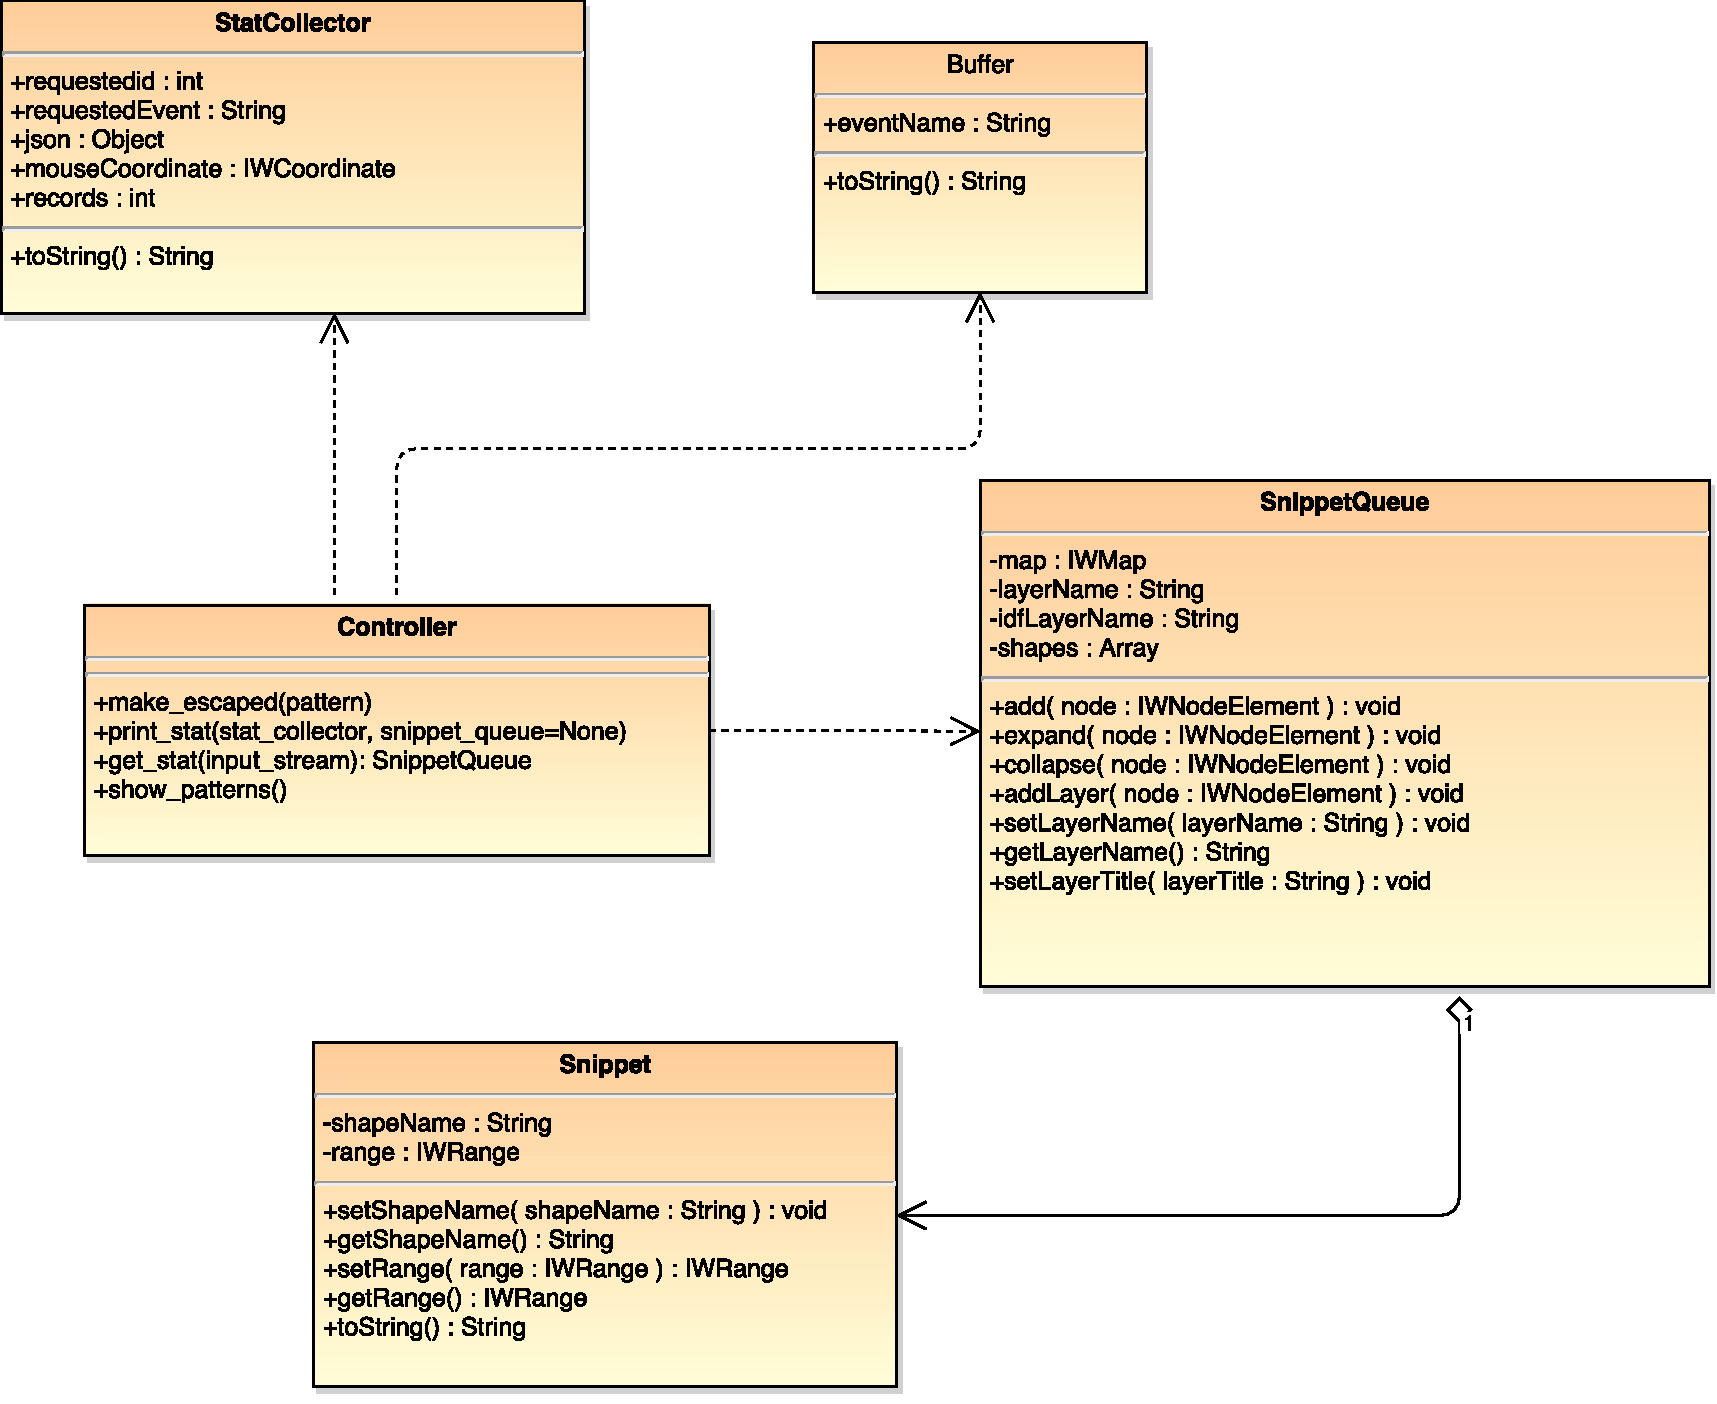
\includegraphics[width=\textwidth]{pics/arch.pdf}
  \caption{Диаграмма классов}
  \label{fig:umlclasses}
\end{figure}

\section{Планируемая выгода}

В настоящий момент из-за сложности ручного анализа файл журналов error\_log,
содержащий большое количество неструктурированной информации и
лишних сообщений используется только в крайних случаях, когда другие
инструменты не дают достаточно информации о проблеме. Инженер затрачивает
от одной до трёх минут на поиск необходимого сообщения с релевантной
информацией.

С помощью разрабатываемого алгоритма можно получить следующие улучшения
существующего процесса:

\begin{itemize}
  \item Можно предоставить информацию для разработчиков, позволяющую провести
    рефакторинг подсистемы вывода сообщений об ошибках, что уменьшит
    количество неинформативных сообщений и улучшит структуру файла журнала.
  \item Позволит исключить неинформативные сообщения без изменения существующих
    приложений из файла журнала и предоставить инженеру максимально
    информативную выжимку.
  \item Позволит дать возможность ручного анализа файла журнала инженерам,
    что уменьшит время диагностики проблем.
  \item Позволит предсказывать нештатные ситуации за счёт регулярного
    автоматического анализ.
\end{itemize}
